\documentclass[onecolumn, draftclsnofoot,10pt, compsoc]{IEEEtran}
\hbadness=1000 % suppress warnings
\usepackage{graphicx}
\usepackage{url}
\usepackage{setspace}
\usepackage{hyperref}
\usepackage{listings}
\usepackage{cite}
\usepackage{geometry}
\usepackage{pdfpages}
\usepackage{longtable}
\include{pygments.tex}

\geometry{textheight=9.5in, textwidth=7in}

% 1. Fill in these details
\def \CapstoneTeamName{		Aerolyzer}
\def \CapstoneTeamNumber{		19}
\def \GroupMemberOne{			Daniel Ross}
\def \GroupMemberTwo{			Logan Wingard}
\def \CapstoneProjectName{		Aerolyzer}
\def \CapstoneSponsorPerson{		Kim Whitehall}


% 2. Uncomment the appropriate line below so that the document type works
\def \DocType{		%Problem Statement
	%Requirements Document
	%Technology Review
	%Design Document
	%Progress Report
	Final Report
}

\newcommand{\NameSigPair}[1]{\par
	\makebox[2.75in][r]{#1} \hfil 	\makebox[3.25in]{\makebox[2.25in]{\hrulefill} \hfill		\makebox[.75in]{\hrulefill}}
	\par\vspace{-12pt} \textit{\tiny\noindent
		\makebox[2.75in]{} \hfil		\makebox[3.25in]{\makebox[2.25in][r]{Signature} \hfill	\makebox[.75in][r]{Date}}}}
% 3. If the document is not to be signed, uncomment the RENEWcommand below
\renewcommand{\NameSigPair}[1]{#1}

%%%%%%%%%%%%%%%%%%%%%%%%%%%%%%%%%%%%%%%
\graphicspath{{images/}}
\begin{document}
	\begin{titlepage}
		\pagenumbering{gobble}
		\begin{singlespace}
			\centering
			
\includegraphics[height=4cm,natwidth=345,natheight=435]{images/coe_v_spot1.png}
			\hfill 
			% 4. If you have a logo, use this includegraphics command to put it on the coversheet.
			%\includegraphics[height=4cm]{CompanyLogo}   
			\par\vspace{.2in}
			\centering
			\scshape{
				\huge CS Capstone \DocType \par
				{\large\today}\par
				\vspace{.5in}
				\textbf{\Huge\CapstoneProjectName}\par
				\vfill
				{\large Prepared for}\par
				{\Large\NameSigPair{\CapstoneSponsorPerson}\par}
				{\large Prepared by }\par
				Group\CapstoneTeamNumber\par
				% 5. comment out the line below this one if you do not wish to name your team
				\CapstoneTeamName\par 
				\vspace{5pt}
				{\large
					\NameSigPair{\GroupMemberOne}\par
					\NameSigPair{\GroupMemberTwo}\par
				}
				\vspace{20pt}
			}
			\begin{abstract}  
				The Aerolyzer Project aims to deliver a new source of air quality and weather information through leveraging existing weather data and image analysis algorithms.
				When complete, this open-source project shall feature a Python library that uses image classification and third-party weather APIs, displayed with an intuitive web-based user interface.
			\end{abstract}     
		\end{singlespace}
	\end{titlepage}

\tableofcontents
\clearpage

\begin{singlespace}

	\section{Introduction}
		Aerolyzer is a project initially proposed by NASA JPL that aims to deliver a new source of air quality and weather information through leveraging existing weather data and image analysis algorithms.
		Though lots had come up on the client's side of the project, and the details are a bit unclear, the client as of the end of the project is Kim Whitehall.
		The posible uses of the Aerolyzer python library include checking weather data to gain aerosol information in order to conclude whether alergy medication may be necessary.
		The project group initially consisted of three members, those members being Logan Wingard, Daniel Ross, and Kin-Ho Lam, though the project group finished with only two, those being Daniel and Logan.
		Kin-Ho Lam's name will be in the previous documents, though was not a part of the project as of winter term.
		Kim Whitehall was in charge of directing and managing the direction the project was going, while Logan and Daniel determined methods problems would be solved, as well as coding and implemeting these solutions.
		
	\section{Requirements Document}
		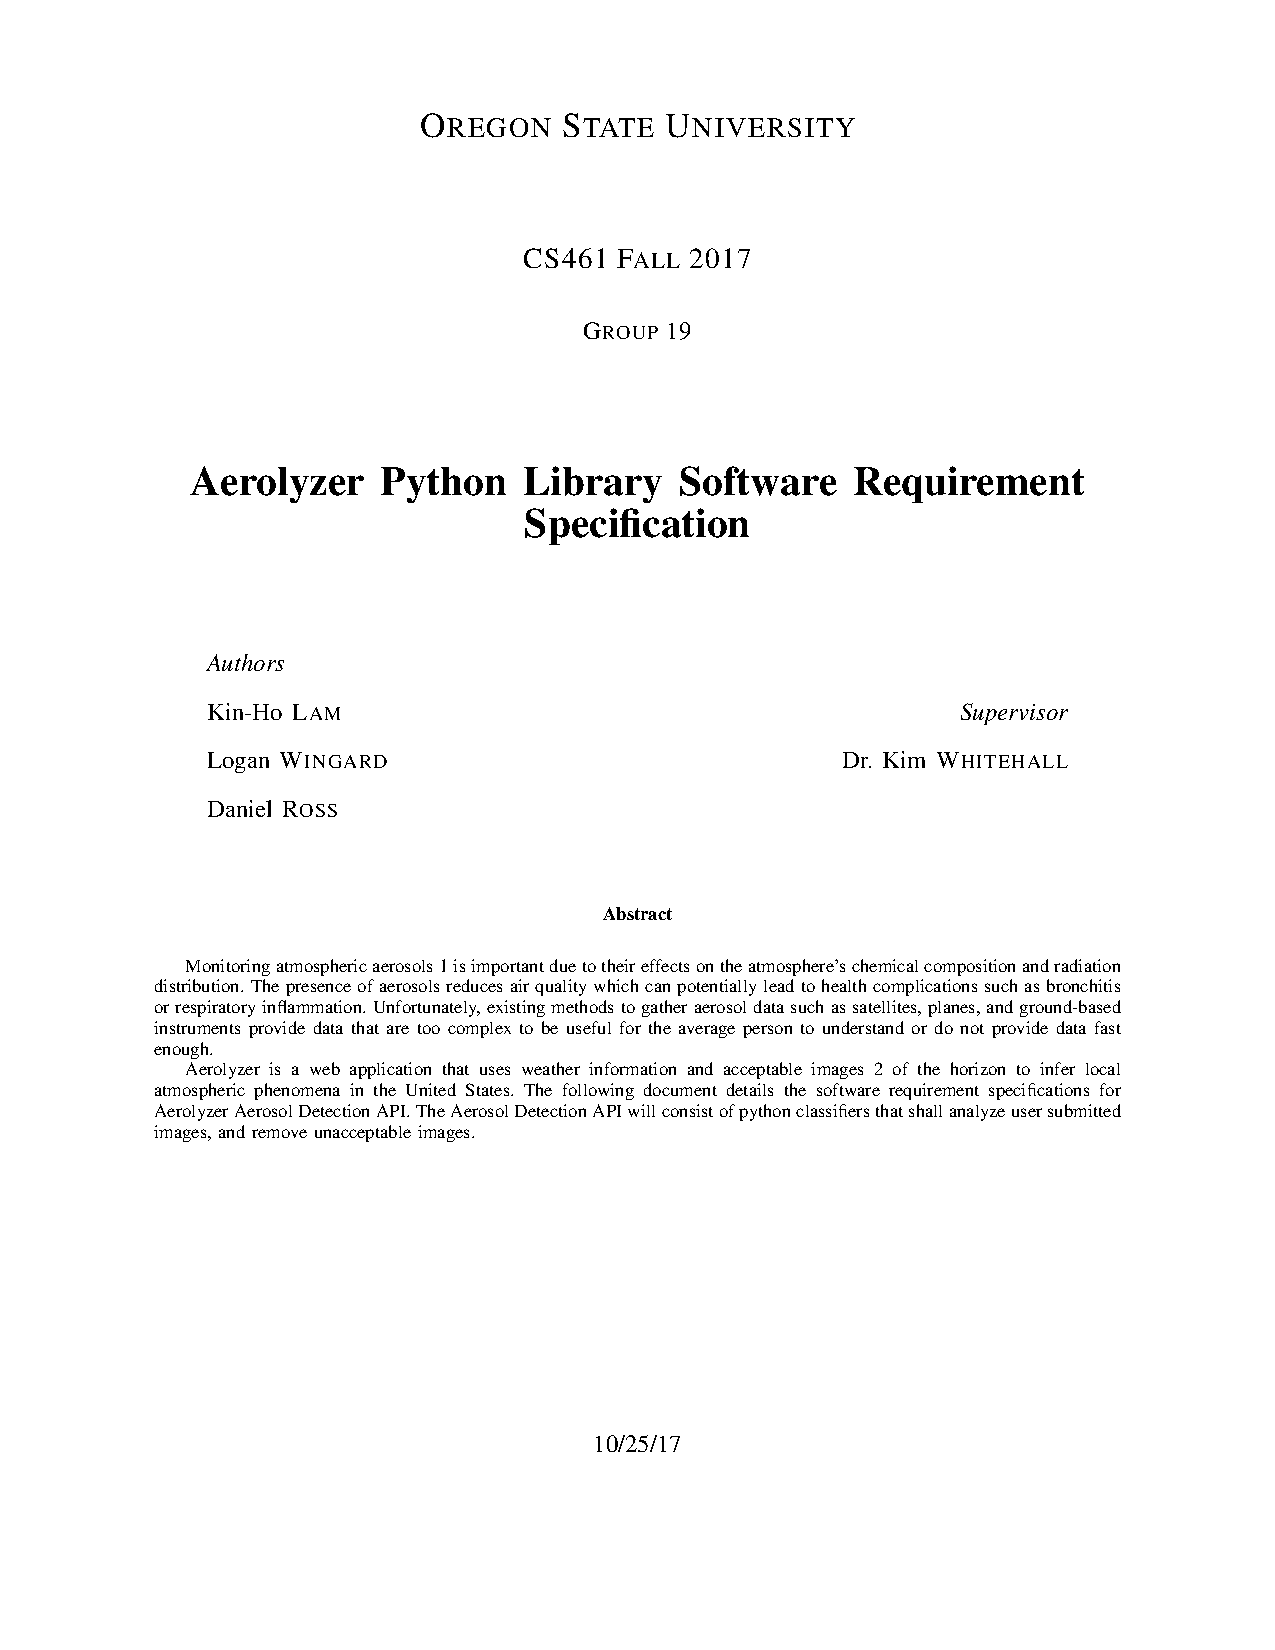
\includepdf[pages=-]{pdfs/require.pdf}
	\section{Design Document}
		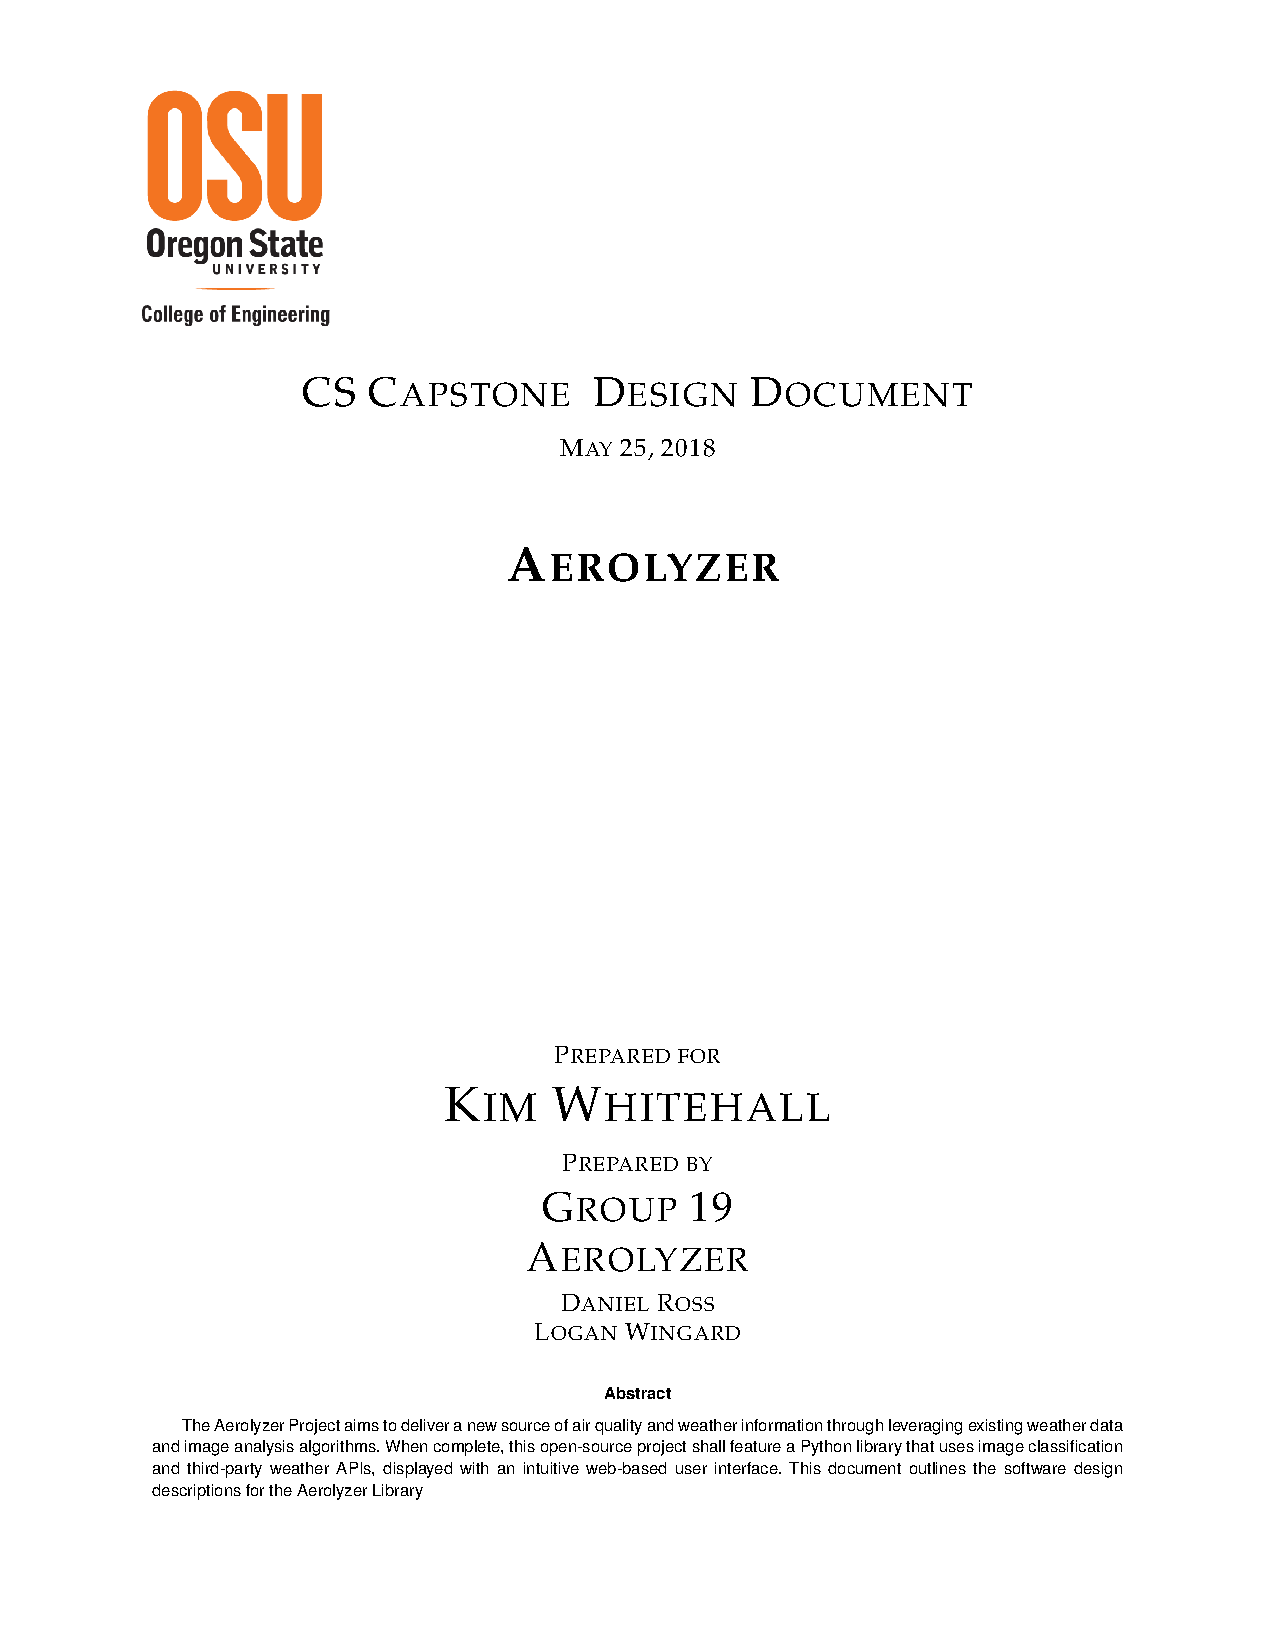
\includepdf[pages=-]{pdfs/design.pdf}
	\section{Tech Review}
		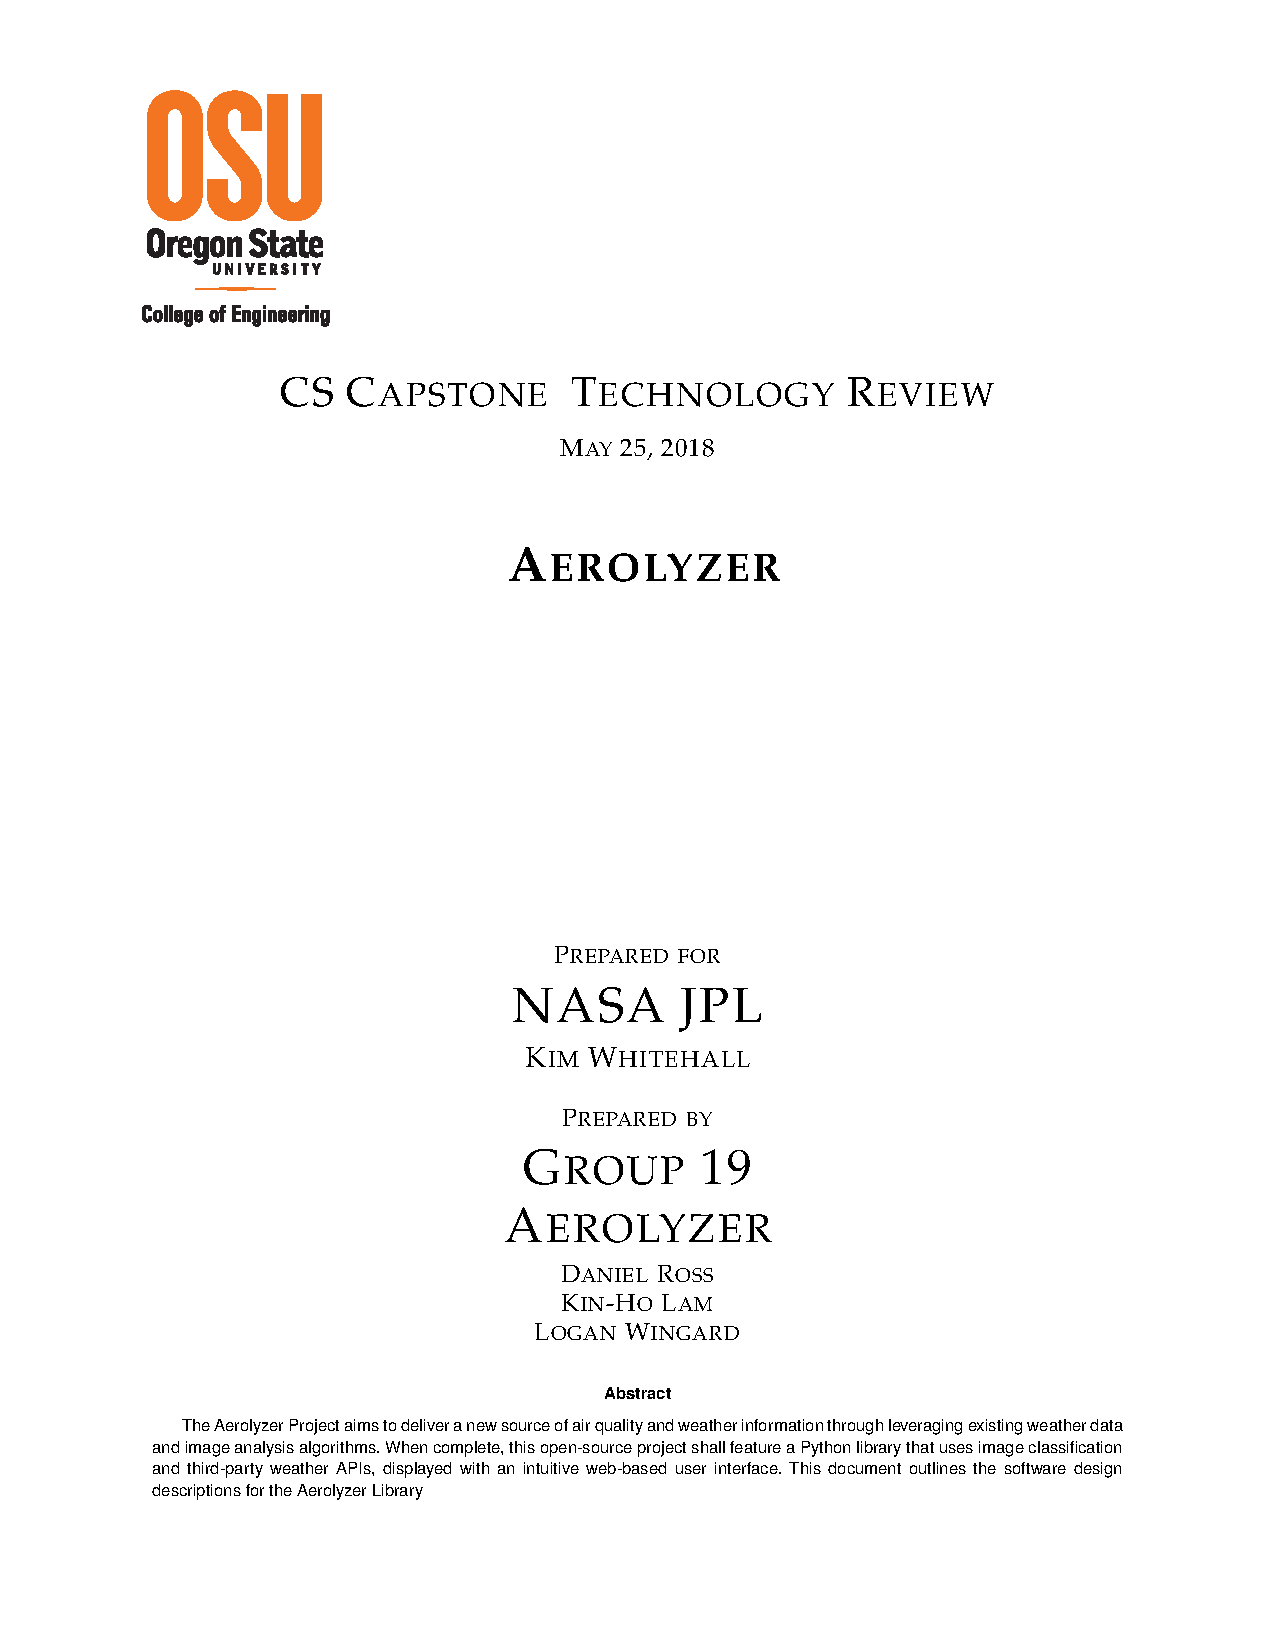
\includepdf[pages=-]{pdfs/tech.pdf}
	\section{Blog Posts}
		\subsection{Daniel Ross}
			\begin{longtable}{|l|p{0.3\linewidth}|p{0.3\linewidth}|p{0.3\linewidth}|}\hline \textbf{Week} & \textbf{Fall} & \textbf{Winter} & \textbf{Spring}\\\hline
			1 & - & - & -
			\\\hline
			2 & - & - & -
			\\\hline
			3 & - & - & -
			\\\hline
			4 & - & - & -
			\\\hline
			5 & - & - & -
			\\\hline
			6 & - & - & -
			\\\hline
			7 & - & - & -
			\\\hline
			8 & - & - & -
			\\\hline
			9 & - & - & -
			\\\hline
			10 & - & - & -
			\\\hline
			
			\end{longtable}
		\subsection{Logan Wingard}
			\begin{longtable}{|l|p{0.3\linewidth}|p{0.3\linewidth}|p{0.3\linewidth}|}\hline \textbf{Week} & \textbf{Fall} & \textbf{Winter} & \textbf{Spring}\\\hline
			1 &
			Set up one note (I think) 
			Looked over projects. Very interested in the 3d vr painting project.
			Reached out to Mike Bailey & One Group member was removed for the group

Kim also mentioned that we were low priority with her new schedule. 
I take this more as a challenge to prove her wrong with some good code output & I have been working on linting, cleaning and testing my code.
I am planning on creating a pull request with these changes soon.
			\\\hline
			2 & 
			Assigned to team 19 Aerolyzer
			Met with client 
			We discussed goals, technicals, and made a plan for the problem statement  & Daniel has written a lon lat conversion function to get it in a more usable format

We need to start making database decisions, what needs to be saved on the database and what doesn't.

We are also informed that we need to remove NASA JPL from all docs, as there is no longer a connection between Aerolyzer and NASA. & Lots of bug testing this week. Through some tests, I found that my accuracy was short by a bit, so I improved my algorithm to rach the desired accuracy
			\\\hline
			3 & 
			Summary: 
			We had another meeting with our client, this one had a focus on project requirements.

			We also met with our TA for the first time :
			Narrow down requirements.
			Bring 3x5 notecard to write requirements down. If it doesn’t fit, narrow down.
			Nail down EXACTLY what client wants
			Don’t be afraid to negotiate with client. 
			Do something silly to familiarize with framework. & Worked a bit on image classification, only to realize most of them have already been completed by the previous group, without our client's or my knowledge.

Daniel has also made great progress on location functions. & We are starting our wired articles. They are basically "reviews" for eachother's projects.

I met with Dennie DeVito in class and we agreed to interview each other for the assignment.
			\\\hline
			4 & We were able to get the problem statement in.
We will look into what the requirements doc is. We've also been experimenting with the vm and opencv & Been working on my code for horizon detection. Still brainstorming about methods do do this. Right now I am able to single out the sky if one is present in an image. Still not very accurate & I emailed dennie again with no response. I contacted Kirsten to let her know about the situation and she informed me another classmate also had a similar issue, which works out great for the both of us. We interviewed each other and were able to write our articles and submit them on time
			\\\hline
			5 & We have a very good draft of the requirements doc. Our rough draft was missing a Ghant chart, though I'm fairly happy with the draft. & I'm having a lot of issues with git. My algorithm for horizon detection is covered over about 30 commits and that is too much to look over for one pull request. Worked on rebasing and linting code to make both the code and the pull request more readable & For an unknown reason, Kim has not been replying to emails. Last meeting, she mentioned that she was not feeling well, so we are hoping eveerything is alright. 

The issue with the config files has hopefully been resolved. When we regain contact with Kim, we will show her our methods and hopefully get some direction. 
			\\\hline
			6 & 
The final requirements doc looks really good. Got a very good looking ghant chart. 
We have still been looking into importing python libraries and how to create one. 
We also found some code that shares many of the functions that we hope to use. We plan on contacting the creator and ask permission. There also has to be edits to the code to actually make it usable, considering the code we found takes in live video while we only need to use it for 1 picture at a time. 
& I've decided to try to implement some machine learning into my horizon detection as I am unable to make the 66\% accuracy goal. Been messing arround with neural networks and I'll see where that leads
 & Kim reconnected with us after a couple weeks of silence and we were able to get back on track.

With her guidance, we decided to combine our two fixes to the config issue and we now have a working library that is ready (hopefully) for expo
			\\\hline
			7 & After looking more into python modules, I was able to get the module set up correctly.
We ended up not using the horizon code that we found because it wasn't very compatible. We are going to try to write one from scratch. & Continued working on Neural network for horizon detection and it reached the 66\% benchmark. That is about all I've been able to work on over the week & When testing our library for expo, I found sevevral bugs that luckily had simple fixes. I have opened a github issue ad I will create a pull request fixing these bugs sometime after expo.

Expo went really well. If anything, we overprepared, going as far as to bring a whiteboard for explanations to really technical questions that were (thankfully) never asked.
			\\\hline
			8 & I messed up when pushing to github and our client is not a happy camper. 
I agreed to have a 1 on 1 with our client to discuss git workflow.  & Cleaning up and linting code before I make a pull request. I'm moving onto color extraction and getting the data from the haze layer to the functions that Daniel has been working on for color analysis & Post expo, it is now time to start working on final documentation. Start getting all the git issues and weekly blogs together for the report, and start putting a script together for our final presentation.
Lastly we will need to fill out peer reviews and sign off the code to our client.
			\\\hline
			9 &  Had a good break. Set a time for meeting with client.  & Color extraction was pretty simble as the code I used to find the horizon was very helpful in singling out the haze layer.  Made it so it will chose 1000 random points to pass to the color analysis. & Not much left to do except keep working on documentation. the code has been completed.
			\\\hline
			10 & We've been working on the design doc. Trying to get that submitted on our team one note. Looks like we won't be able to start our progress reports until the weekend.  & The only thing I'm really able to work on this week has been the progress report. Will get that writen up, recorded and submitted & We finished and submitted our final presentation, all that is left to do is finish with this report.
			\\\hline
			
			\end{longtable}
	\section{Poster}
		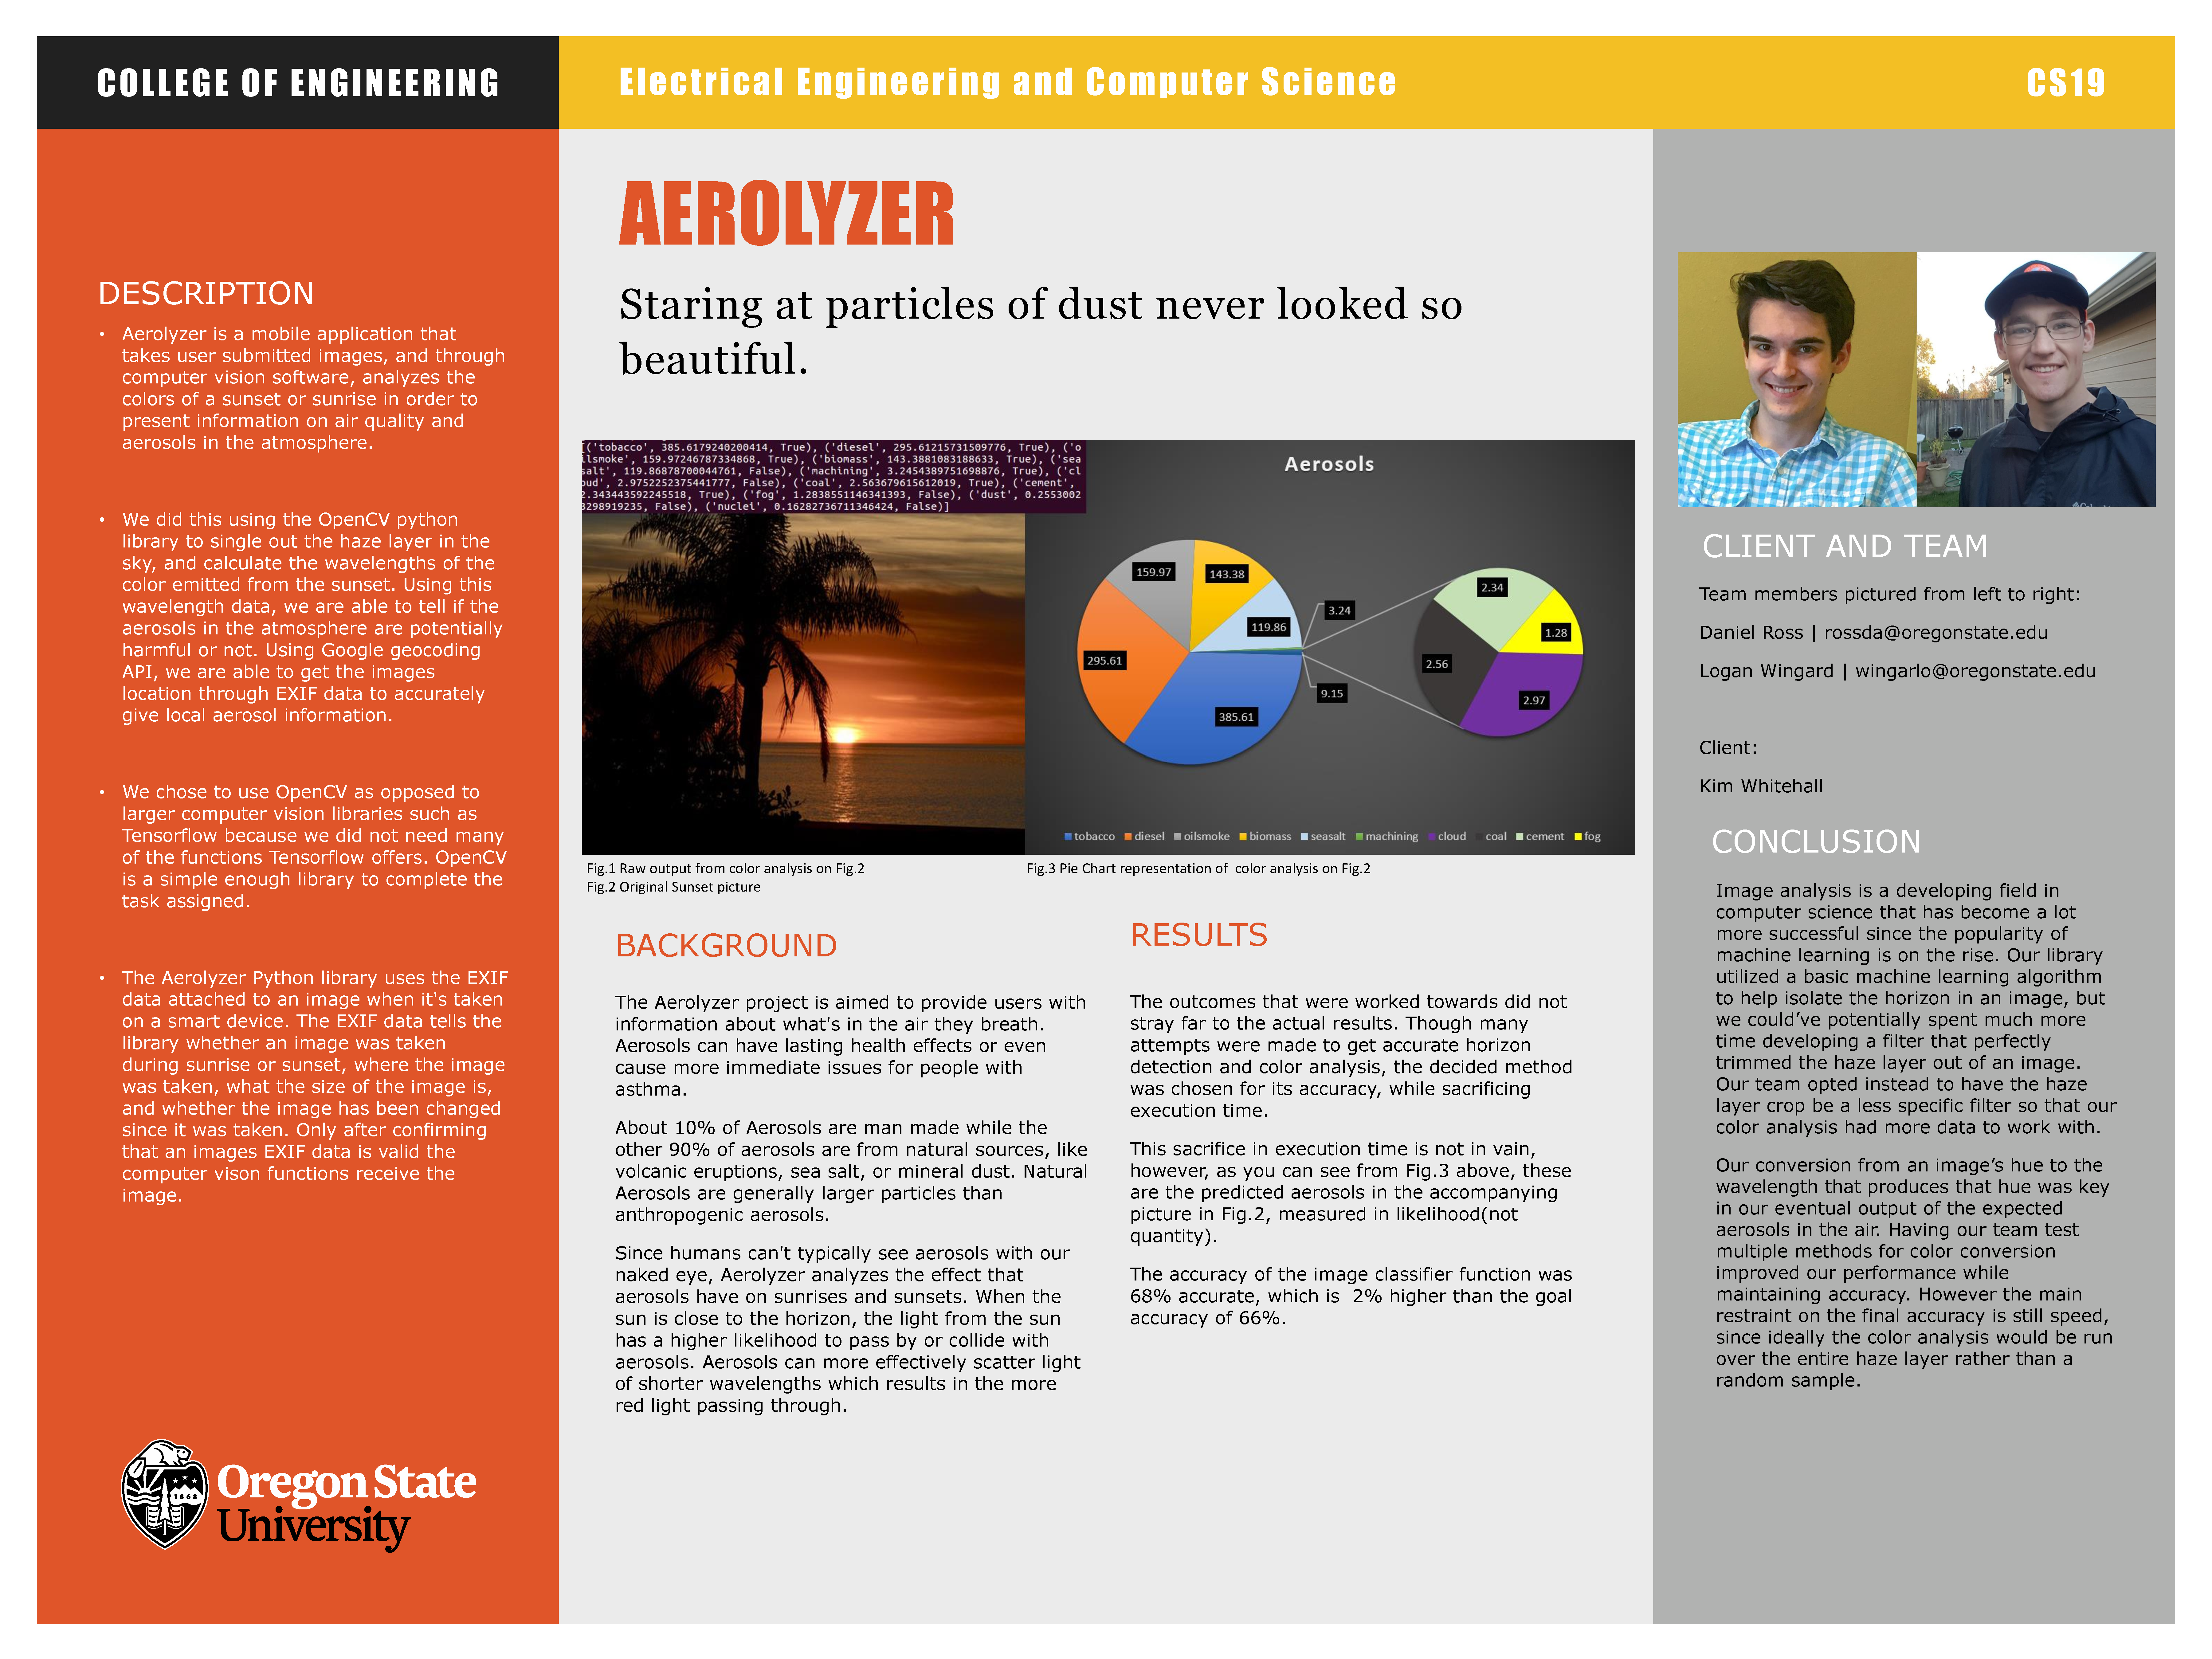
\includepdf[pages=-]{pdfs/poster.pdf}
	\section{Project Documentations}
		todo
	\section{Recommended Resources for Learning More}
		Aerolyzer is completely open source and is even on the Python Package Index (pypi).
		To learn more about how Aerolyzer works, all the code and documentation is on the Aerolyzer github.
		Some of the resources used to learn the techniques implemented into the Aerolyzer library include the following.
		Neural networks:\\
		\url{https://github.com/llSourcell/Make_a_neural_network/blob/master/demo.py} \\
		\url{https://iamtrask.github.io/2015/07/12/basic-python-network/} \\

		Aerosols:\\
		\url{https://aeronet.gsfc.nasa.gov/new_web/Documents/Aerosol_Optical_Depth.pdf} \\

		Pypi:\\
		\url{https://packaging.python.org/tutorials/distributing-packages/#setup-py} \\
		
		Color information: \\
		\url{https://www.weather.gov/jetstream/color} \\
		\url{https://en.wikipedia.org/wiki/File:Linear_visible_spectrum.svg} \\
		\url{http://steve.hollasch.net/cgindex/color/freq-rgb.html} \\
		\url{http://www.efg2.com/Lab/ScienceAndEngineering/Spectra.html} \\
		\url{http://www.physics.sfasu.edu/astro/color/spectra.html} \\

		This is the code that was used to generate the image being used. \\
		\url{http://www.gringene.org/code/spectrum.r} \\


	\section{Conclusion}
		todo \cite{neural}
	\section{Appendix}
		todo
\end{singlespace}
\clearpage
\bibliographystyle{IEEEtran}
\bibliography{ref}
\end{document}
